% =============================================================================
% CHAPITRE 1 - CINÉMATIQUE
% Partie 8 : Chute libre
% Version maritime pour l'IMQ
% =============================================================================

% =============================================================================
\section{Corps en chute libre}
% =============================================================================

La chute libre est un cas particulier tr\`es important du MRUA : c'est le mouvement d'un objet soumis uniquement \`a la gravit\'e. Ce type de mouvement est omnipr\'esent, que ce soit un outil qui tombe d'un m\^at, un plongeur qui saute \`a l'eau, ou un homme \`a la mer.

\begin{remarque}[title=Questions types que nous allons r\'esoudre]
Dans cette section, vous apprendrez \`a r\'epondre aux questions suivantes :
\begin{itemize}
    \item Combien de temps dure une chute d'une hauteur donn\'ee?
    \item \`A quelle vitesse un objet touche-t-il le sol (ou l'eau)?
    \item Quelle hauteur maximale atteint un objet lanc\'e vers le haut?
    \item Combien de temps un objet lanc\'e vers le haut reste-t-il en l'air?
    \item Quelle vitesse initiale faut-il pour atteindre une certaine hauteur?
\end{itemize}
\end{remarque}

\subsection{D\'efinition et hypoth\`eses}

\begin{definition}[title=Chute libre]
Un \textbf{corps en chute libre} est un objet qui se d\'eplace uniquement sous l'influence de la gravit\'e, sans qu'aucune autre force n'agisse sur lui de fa\c{c}on significative.

\textbf{Attention :} Un corps en chute libre n'est pas n\'ecessairement un objet qui \guillemotleft~tombe~\guillemotright. Un objet lanc\'e vers le haut est aussi en chute libre d\`es qu'il quitte la main!
\end{definition}

\begin{remarque}[title=Hypoth\`eses simplificatrices]
Pour \'etudier la chute libre, on fait deux hypoth\`eses :
\begin{enumerate}
    \item La \textbf{r\'esistance de l'air est n\'egligeable} (valable pour des objets denses \`a faible vitesse)
    \item L'\textbf{altitude reste faible} par rapport au rayon de la Terre (donc $g$ est constante)
\end{enumerate}
Ces hypoth\`eses permettent de traiter la chute libre comme un \textbf{MRUA vertical}.
\end{remarque}

\subsection{L'acc\'el\'eration gravitationnelle}

Pr\`es de la surface de la Terre, tous les corps en chute libre subissent la m\^eme acc\'el\'eration, quelle que soit leur masse :

\begin{equationimportante}
\begin{equation}
g = \SI{9,81}{m/s^2} \quad \text{(vers le centre de la Terre)}
\end{equation}
\end{equationimportante}

\begin{exemple}{Exp\'erience historique : la plume et le marteau}{}
Le 2 ao\^ut 1971, l'astronaute David Scott a r\'ealis\'e une exp\'erience sur la Lune : il a l\^ach\'e simultan\'ement un marteau de g\'eologue et une plume de faucon. Sans atmosph\`ere pour cr\'eer de la r\'esistance, les deux objets sont arriv\'es au sol \textbf{en m\^eme temps}, confirmant que tous les corps tombent avec la m\^eme acc\'el\'eration en l'absence d'air.

Sur Terre, une plume tombe plus lentement qu'un marteau \`a cause de la r\'esistance de l'air, pas \`a cause d'une diff\'erence d'acc\'el\'eration gravitationnelle.

\begin{center}
\textit{Visionnez cette exp\'erience historique :}\\[0.3em]
\url{https://www.youtube.com/watch?v=KDp1tiUsZw8}
\end{center}
\end{exemple}

\subsection{Convention de signes}

Le choix de l'orientation de l'axe $y$ détermine le signe de l'accélération :

\begin{center}
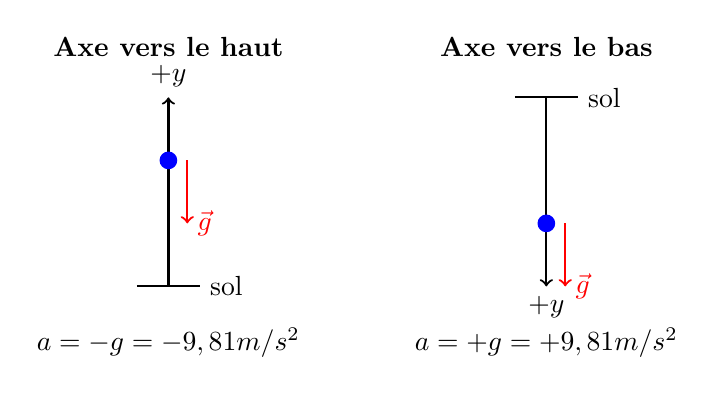
\begin{tikzpicture}[scale=0.8]
% Cas 1 : y vers le haut
\begin{scope}[shift={(0,0)}]
\draw[thick, ->] (0,0) -- (0,3) node[above] {$+y$};
\draw[thick] (-0.5,0) -- (0.5,0) node[right] {sol};
\fill[blue] (0,2) circle (4pt);
\draw[thick, red, ->] (0.3,2) -- (0.3,1) node[right] {$\vec{g}$};
\node[below] at (0,-0.5) {$a = -g = \SI{-9,81}{m/s^2}$};
\node[above] at (0,3.5) {\textbf{Axe vers le haut}};
\end{scope}
% Cas 2 : y vers le bas
\begin{scope}[shift={(6,0)}]
\draw[thick, ->] (0,3) -- (0,0) node[below] {$+y$};
\draw[thick] (-0.5,3) -- (0.5,3) node[right] {sol};
\fill[blue] (0,1) circle (4pt);
\draw[thick, red, ->] (0.3,1) -- (0.3,0) node[right] {$\vec{g}$};
\node[below] at (0,-0.5) {$a = +g = \SI{+9,81}{m/s^2}$};
\node[above] at (0,3.5) {\textbf{Axe vers le bas}};
\end{scope}
\end{tikzpicture}
\end{center}

\begin{attention}
La convention la plus courante (et celle utilisée dans ce cours) est de choisir l'axe $y$ \textbf{positif vers le haut}. Dans ce cas :
\[ a_y = -g = \SI{-9,81}{m/s^2} \]
Le signe négatif indique que l'accélération est dirigée vers le bas.
\end{attention}

\subsection{Équations de la chute libre}

Les équations de la chute libre sont les équations du MRUA appliquées à la direction verticale :

\begin{equationimportante}
\textbf{Équations de la chute libre} (axe $y$ positif vers le haut)
\begin{align}
v_y &= v_{iy} + a_y \Delta t = v_{iy} - g\Delta t \\[0.3cm]
\Delta y &= v_{iy} \Delta t + \frac{1}{2}a_y (\Delta t)^2 = v_{iy} \Delta t - \frac{1}{2}g(\Delta t)^2 \\[0.3cm]
v_y^2 &= v_{iy}^2 + 2a_y \Delta y = v_{iy}^2 - 2g\Delta y
\end{align}
\end{equationimportante}

\begin{remarque}[title=Notation]
\begin{itemize}
    \item $v_{iy}$ : vitesse initiale verticale (positive vers le haut, négative vers le bas)
    \item $v_y$ : vitesse finale verticale
    \item $\Delta y = y_f - y_i$ : déplacement vertical
    \item $g = \SI{9,81}{m/s^2}$ : valeur absolue de l'accélération gravitationnelle
\end{itemize}
\end{remarque}

\subsection{Cas particuliers}

\subsubsection{Objet lâché (sans vitesse initiale)}

\begin{exemple}{Outil tombant d'un mât (exemple maritime)}{}
Un matelot échappe une clé à molette du haut d'un mât situé à $\SI{25}{m}$ au-dessus du pont. 
\begin{enumerate}[label=\alph*)]
    \item Combien de temps met la clé pour atteindre le pont?
    \item À quelle vitesse frappe-t-elle le pont?
\end{enumerate}

\textbf{Données :}
\begin{itemize}
    \item $y_i = \SI{25}{m}$ (origine au pont, axe vers le haut)
    \item $y_f = \SI{0}{m}$
    \item $v_{iy} = \SI{0}{m/s}$ (lâchée, pas lancée)
    \item $a_y = \SI{-9,81}{m/s^2}$
\end{itemize}

\textbf{a) Temps de chute :}
\begin{align*}
\Delta y &= v_{iy} \Delta t - \frac{1}{2}g(\Delta t)^2 \\
0 - 25 &= 0 - \frac{1}{2}(9,81)(\Delta t)^2 \\
\Delta t &= \sqrt{\frac{2 \times 25}{9,81}} = \SI{2,26}{s}
\end{align*}

\textbf{b) Vitesse d'impact :}
\begin{align*}
v_y &= v_{iy} - g\Delta t \\
v_y &= 0 - 9,81 \times 2,26 = \SI{-22,2}{m/s}
\end{align*}

Le signe négatif indique que la vitesse est dirigée vers le bas. La clé frappe le pont à $\SI{22,2}{m/s}$ ($\SI{80}{km/h}$)!

\begin{attention}
C'est pourquoi le port du casque est obligatoire sur les chantiers navals et lors de certaines opérations à bord!
\end{attention}
\end{exemple}

\begin{pratiqueautonome}
Un conteneur se détache d'une grue portuaire et tombe d'une hauteur de $\SI{18}{m}$ au-dessus du quai.

\begin{enumerate}[label=\alph*)]
    \item Combien de temps dure la chute?
    \item À quelle vitesse le conteneur frappe-t-il le quai? Exprimez votre réponse en m/s et en km/h.
\end{enumerate}

\espaceresolution[6cm]
\reponsepratique{a) $\Delta t \approx \SI{1,9}{s}$ \quad b) $v \approx \SI{18,8}{m/s} \approx \SI{68}{km/h}$}
\end{pratiqueautonome}

\subsubsection{Objet lancé vers le haut}

\begin{exemple}{Fusée éclairante lancée à la main}{}
Un marin lance une fusée éclairante vers le haut avec une vitesse initiale de $\SI{15}{m/s}$ depuis le pont situé à $\SI{8}{m}$ au-dessus de l'eau.
\begin{enumerate}[label=\alph*)]
    \item Quelle hauteur maximale atteint-elle?
    \item Combien de temps reste-t-elle en l'air avant de toucher l'eau?
\end{enumerate}

\textbf{Données :}
\begin{itemize}
    \item $y_i = \SI{8}{m}$ (origine à la surface de l'eau)
    \item $v_{iy} = \SI{+15}{m/s}$ (vers le haut)
    \item $a_y = \SI{-9,81}{m/s^2}$
\end{itemize}

\textbf{a) Hauteur maximale :}

Au point le plus haut, la vitesse verticale est nulle ($v_y = 0$).
\begin{align*}
v_y^2 &= v_{iy}^2 - 2g\Delta y \\
0 &= 15^2 - 2(9,81)\Delta y \\
\Delta y &= \frac{225}{19,62} = \SI{11,5}{m}
\end{align*}

Hauteur maximale : $y_{max} = y_i + \Delta y = 8 + 11,5 = \SI{19,5}{m}$ au-dessus de l'eau.

\textbf{b) Temps total en l'air :}

La fusée touche l'eau quand $y_f = 0$.
\begin{align*}
y_f &= y_i + v_{iy} \Delta t - \frac{1}{2}g(\Delta t)^2 \\
0 &= 8 + 15\Delta t - 4,905(\Delta t)^2
\end{align*}

Équation quadratique : $4,905(\Delta t)^2 - 15\Delta t - 8 = 0$

\[ \Delta t = \frac{15 \pm \sqrt{225 + 4(4,905)(8)}}{2(4,905)} = \frac{15 \pm 18,5}{9,81} \]

Solution positive : $\Delta t = \SI{3,41}{s}$

La fusée reste en l'air pendant $\SI{3,41}{s}$.
\end{exemple}

\begin{pratiqueautonome}
Un marin lance verticalement une bouée de sauvetage lumineuse avec une vitesse initiale de $\SI{12}{m/s}$ depuis le pont situé à $\SI{6}{m}$ au-dessus de l'eau.

\begin{enumerate}[label=\alph*)]
    \item Quelle hauteur maximale atteint-elle au-dessus de l'eau?
    \item Combien de temps reste-t-elle en l'air avant de toucher l'eau?
\end{enumerate}

\textit{Indice : Pour a), au point le plus haut, $v_y = 0$. Pour b), résolvez $y_f = 0$.}

\espaceresolution[7cm]
\reponsepratique{a) $y_{max} \approx \SI{13,3}{m}$ \quad b) $\Delta t \approx \SI{2,8}{s}$}
\end{pratiqueautonome}

\begin{remarque}[title=Symétrie de la chute libre]
Pour un objet lancé vers le haut qui retombe au même niveau :
\begin{itemize}
    \item Le temps de montée égale le temps de descente
    \item La vitesse de retour a la même grandeur que la vitesse initiale (mais sens opposé)
\end{itemize}
Cette symétrie ne s'applique que si le point de départ et d'arrivée sont au même niveau.
\end{remarque}

\subsection{Application maritime : homme à la mer}

\begin{exemple}{Chute d'un homme à la mer}{}
Un marin tombe d'un pont situé à $\SI{12}{m}$ au-dessus de la surface de l'eau. En supposant qu'il ne saute pas (vitesse initiale nulle) :
\begin{enumerate}[label=\alph*)]
    \item Combien de temps dure la chute?
    \item À quelle vitesse entre-t-il dans l'eau?
\end{enumerate}

\textbf{a) Temps de chute :}
\[ \Delta t = \sqrt{\frac{2h}{g}} = \sqrt{\frac{2 \times 12}{9,81}} = \SI{1,56}{s} \]

\textbf{b) Vitesse d'entrée dans l'eau :}
\[ v = g \Delta t = 9,81 \times 1,56 = \SI{15,3}{m/s} \approx \SI{55}{km/h} \]

\begin{attention}
Une entrée dans l'eau à $\SI{55}{km/h}$ peut causer des blessures graves si la position du corps n'est pas adéquate. C'est pourquoi la formation à la survie en mer insiste sur la position à adopter lors d'une chute : bras croisés, jambes serrées, regard à l'horizon.
\end{attention}
\end{exemple}

\begin{center}
\renewcommand{\arraystretch}{1.5}
\begin{tabular}{|c|c|c|}
\hline
\rowcolor{bleuclair}
\textbf{Hauteur de chute} & \textbf{Temps de chute} & \textbf{Vitesse d'impact} \\
\hline
$\SI{5}{m}$ & $\SI{1,0}{s}$ & $\SI{10}{m/s}$ ($\SI{36}{km/h}$) \\
\hline
$\SI{10}{m}$ & $\SI{1,4}{s}$ & $\SI{14}{m/s}$ ($\SI{50}{km/h}$) \\
\hline
$\SI{15}{m}$ & $\SI{1,7}{s}$ & $\SI{17}{m/s}$ ($\SI{62}{km/h}$) \\
\hline
$\SI{20}{m}$ & $\SI{2,0}{s}$ & $\SI{20}{m/s}$ ($\SI{72}{km/h}$) \\
\hline
$\SI{30}{m}$ & $\SI{2,5}{s}$ & $\SI{24}{m/s}$ ($\SI{87}{km/h}$) \\
\hline
\end{tabular}
\end{center}

\begin{remarque}[title=L'universalité de la chute libre]
Les équations de la chute libre s'appliquent à tout objet : un conteneur qui tombe d'une grue, un plongeur qui saute d'un tremplin, une pomme qui tombe d'un arbre, ou une balle lancée en l'air. Seule la valeur de $g$ change selon la planète!

Sur la Lune : $g_{Lune} = \SI{1,62}{m/s^2}$ (environ 6 fois moins que sur Terre).
\end{remarque}
